\section{More about Rings and Modules}
In this section, we shall introduce some more concepts and properties about rings and ideals.
\subsection{Further Topics on Rings and Ideals}
This section mainly deal with rings. As mentioned in the preface of this part, we only deal with commutative rings unless stated otherwise.
\begin{center}
\begin{large}
    \textbf{Nilradical and Jacobson Radical}
\end{large}
\end{center}
We begin by considering the following proposition: 
\begin{proposition}
The set $\mathfrak{N}$ of all nilpotent elements in a ring $A$ is an ideal, and $A/\mathfrak{N}$ has no nilpotent element $\ne 0$.
\end{proposition}
\begin{proof}
If $x\in\mathfrak{N}$, then there exists some $n\in\mathbb{Z}$ such that $x^n=0$. Therefore for all $a\in A$ we have $(ax)^n=0$. Now it suffices to show that if $x,y\in\mathfrak{N}$, we have $x^m=0$ and $y^n=0$ for some $m,n\in\mathbb{Z}$. Consider $(x+y)^{m+n+1}$, by the binomial theorem (which is valid for commutative rings), we know that $(x+y)^{m+n+1}$ is a sum of $x^sy^t$ with $s+t=m+n+1$. Therefore there must exists $s>m$ or $t>n$, which implies $x+y\in\mathfrak{N}$ and hence $\mathfrak{N}$ an ideal of $A$.\par
Now we show that there are no nilpotent elements in $A/\mathfrak{N}$. Let $a+\mathfrak{N}\in A/\mathfrak{N}$. Suppose there exists some $n\in\mathbb{Z}$ such that $a^n+\mathfrak{N}=0$, then $a^n\in\mathfrak{N}$, whence $a^{nk}=0$ for some $k\in\mathbb{Z}$. This implies $a\in\mathfrak{N}$ and hence the only nilpotent element in $A/\mathfrak{N}$ is $0$.
\end{proof}
The ideal $\mathfrak{N}$ as defined in Proposition 7.1 is called the \textbf{nilradical} of $A$. The following proposition gives an alternative definition of $\mathfrak{N}$:
\begin{proposition}
The nilradical of $A$ is the intersection of all the prime ideals of $A$.
\end{proposition}
\begin{proof}
Let $\mathfrak{P}$ be the set of all prime ideals of $A$ and $\mathfrak{N}=\bigcap_{\mathfrak{p}\in\mathfrak{P}}\mathfrak{p}$. Let $f\in\mathfrak{N}$, then there exists some $n\in\mathbb{Z}$ such that $f^m=0\in\mathfrak{p}$. Since $\mathfrak{p}$ is prime, we have $f\in\mathfrak{p}$. Note that this is true for all $\mathfrak{p}\in\mathfrak{P}$, we have proved $\mathfrak{N}\subset\mathfrak{N}^\prime$. To prove another direction, let $f\notin\mathfrak{N}$. Then for all $n\in\mathbb{Z}$ we have $f^n\ne 0$. Define $\Sigma$ be the set of all ideals $\mathfrak{a}$ of $A$ such that for all $n>0$, $f^n\notin\mathfrak{a}$. Consider $(\Sigma,\subset)$, which by Zorn's lemma, has a maximal element, denote as $\mathfrak{p}$. We shall show $\mathfrak{p}$ is a prime ideal. If not, then there exists some $x,y\notin\mathfrak{p}$ while $xy\in\mathfrak{p}$. Consider the ideals $\mathfrak{p}+(x)$ and $\mathfrak{p}+(y)$, which strictly include the ideal $\mathfrak{p}$ and hence not in $\Sigma$. Therefore there exists $m,n\in\mathbb{Z}$ such that $f^m\in\mathfrak{p}+(x)$ and $f^n\in\mathfrak{p}+(y)$. This implies $f^{m+n}\in\mathfrak{p}+(xy)$, hence the ideal $\mathfrak{p}+(xy)$ is not in $\Sigma$ and $xy\notin\mathcal{p}$, a contradiction! Therefore $\mathfrak{p}$ is a prime ideal and $f\notin\mathfrak{p}$. Therefore for all $f\notin\mathfrak{N}$ we have $f\notin\mathfrak{N}^\prime$, therefore $\mathfrak{N}^\prime\subset\mathfrak{N}$ and hence $\mathfrak{N}=\mathfrak{N}^\prime$.
\end{proof}
The \textbf{Jacobson radical} $\mathfrak{R}$ is defined to be the intersection of all the maximal ideals of $A$. It can be characterized as follows:
\begin{proposition}
Let $\mathfrak{R}$ be the Jacobson radical of the ring $A$, then $x\in\mathfrak{R}$ if and only if $1-xy$ is a unit in $A$ for all $y\in A$.
\end{proposition}
\begin{proof}
Suppose $x\in\mathfrak{R}$. Then if $1-xy$ is not a unit, we have $1-xy\in\mathfrak{m}$ for some maximal ideals $\mathfrak{m}$. Note that $x\in\mathfrak{m}$, therefore $xy\in\mathfrak{m}$ and hence $1\in\mathfrak{m}$, a contradiction! Conversely, if $x\notin\mathfrak{m}$ for some maximal ideal $\mathfrak{m}$. Then the ideal generated by $\mathfrak{m}$ and $x$ is the unit ideal $(1)$. Therefore there exists some $u\in\mathfrak{m}$ and $y\in A$ such that $u+xy=1$, whence $1-xy=u\in\mathfrak{m}$, and hence $1-xy$ is not a unit.
\end{proof}
\begin{center}
\begin{large}
    \textbf{Operations on Ideals}
\end{large}
\end{center}
Recall that the intersection of any family of ideals is an ideal, the product of any family of ideals, which, when there are only two ideals $\mathfrak{a}$ and $\mathfrak{b}$, is defined to be the set of all finite sums $\sum x_iy_i$ with $x_i\in\mathfrak{a}$ and $y_i\in\mathfrak{b}$. The general case may be defined by (possibly transfinite) induction. In particular, if $\mathfrak{a}$ is an ideal, then $\mathfrak{a}^n$ is defined to be the ideal generated by all elements of the form $x_1x_2\cdots x_n$ with each $x_i\in\mathfrak{a}$. Conventionally we denote $\mathfrak{a}^0=1$.
\begin{example}\em
(i) If $A=\mathbb{Z}$, $\mathfrak{a}=(m)$ and $\mathfrak{b}=(n)$, then $\mathfrak{a}\cap\mathfrak{b}$ is the ideal generated by the l.c.m. of $a$ and $b$, and $\mathfrak{a}\mathfrak{b}=(mn)$. Thus in this case $\mathfrak{a}\mathfrak{b}=\mathfrak{a}\cap\mathfrak{b}$ if and only if $m$ and $n$ are coprime.\par
(ii) Let $A=k[x_1,\cdots,x_n]$ and $\mathfrak{a}=(x_1,\cdots,x_n)$ be the ideal generated by $x_1,\cdots,x_n$. Then $\mathfrak{a}^m$ is the set of all polynomials with no terms of degree $<m$.
\end{example}
Two ideals are said to be \textbf{coprime} if $\mathfrak{a}+\mathfrak{b}=(1)$. Therefore for coprime ideals we have $\mathfrak{a}\cap\mathfrak{b}=\mathfrak{a}\mathfrak{b}$. Clearly two ideals $\mathfrak{a}$, $\mathfrak{b}$ are coprime if and only if there exist $x\in\mathfrak{a}$ and $y\in\mathfrak{b}$ such that $x+y=1$. In general, we have the following: 
\begin{proposition}
Let $A$ be a ring and $\mathfrak{a}_1,\cdots,\mathfrak{a}_n$ are ideals of $A$.Define a homomorphism 
$$
\phi :A\rightarrow \bigoplus_{i=1}^n{\left( A/\mathfrak{a} _i \right)}
$$
by the rule $x\mapsto (x+\mathfrak{a}_1,\cdots,x+\mathfrak{a}_n$.\par
(i) If $\mathfrak{a}_i$ and $\mathfrak{a}_j$ are coprime when $i\ne j$, then $\prod\mathfrak{a}_i=\bigcap\mathfrak{a}_i$.\par
(ii) $\phi$ is surjective if and only if $\mathfrak{a}_i$ and $\mathfrak{a}_j$ are coprime when $i\ne j$, and $\phi$ is injective if and only if $\bigcap\mathfrak{a}_i=(0)$.
\end{proposition}
\begin{proof}
(i) We prove by induction. Suppose $\mathfrak{a}_i$ and $\mathfrak{a}_j$ coprime, we first show that $\mathfrak{a}_i\mathfrak{a}_j=\mathfrak{a}_i\cap\mathfrak{a}_j$. Trivially $\mathfrak{a}_i\mathfrak{a}_j\subset\mathfrak{a}_i\mathfrak{a}_j$. For the converse inclusion, let $x_i\in\mathfrak{a}_i$ and $x_j\in\mathfrak{a}_j$ such that $x_i+x_j=1$. Then $x=xx_i+xx_j\in\mathfrak{a}_i\mathfrak{a}_j$. To prove the general case, suppose the result is true for $k<n$. Therefore suppose $\mathfrak{a}_1,\cdots,\mathfrak{a}_k$ are pairwise coprime, define $\mathfrak{b}=\prod_{i=1}^k\mathfrak{a}_i=\bigcap_{i=1}^k\mathfrak{a}_i$. Since $\mathfrak{a}_i+\mathfrak{a}_k=(1)$ we have $x_i\in\mathfrak{a}_i,y_i\in\mathfrak{a}_k$ such that $x_i+y_i=1$. Therefore 
$$
\prod_{i=1}^{k-1}{x_i}=\prod_{i=1}^{k-1}{\left( 1-y_i \right)}\equiv 1\left( \mathrm{mod}\ \mathfrak{a} _k \right) .
$$
Hence $x=\prod_{i=1}^{k-1}x_i-1\in\mathfrak{a}_k$, whence there exists some $-y\in\mathfrak{a}_k$ such that $x-1=-y$, therefore $x+y=1$ and hence $\mathfrak{a}_k$ and $\mathfrak{b}$ coprime. Therefore 
$$
\mathfrak{b} \mathfrak{a} _k=\left( \prod_{i=1}^{k-1}{\mathfrak{a} _i} \right) \mathfrak{a} _k=\prod_{i=1}^k{\mathfrak{a} _i}=\left( \bigcap_{i=1}^{k-1}{\mathfrak{a} _i} \right) \cap \mathfrak{a} _k=\bigcap_{i=1}^k{\mathfrak{a} _k}.
$$
The proof is therefore finished via induction.\par
(ii) We first note that $\mathrm{Ker}\phi=\bigcap\mathfrak{a}_i$, therefore $\bigcap\mathfrak{a}_i=(0)$ if and only if $\phi$ is surjective. To prove the last condition, we first suppose $\phi$ surjective. We show that $\mathfrak{a}_i$ and $\mathfrak{a}_j$ are coprime. Let $x\in A$ such that 
$$
\phi \left( x \right) =\left( 0,\cdots ,1+\mathfrak{a} _i,\cdots ,0 \right) ,
$$
then $1-x\in\mathfrak{a}_i$ and $x\in\mathfrak{a}_j$. Therefore $1=1-x+x\in\mathfrak{a}_i+\mathfrak{a}_j$. Conversely, suppose $\mathfrak{a}_i$ and $\mathfrak{a}_j$ coprime when $i\ne j$. Then $\mathfrak{a}_i$ is coprime with $\prod_{j\ne i}\mathfrak{a}_j$. Let $x_i\in\mathfrak{a}_i$ and $y_i\in\prod_{j\ne i}\mathfrak{a}_j$ such that $x_i+y_i=1$, therefore $y_i\equiv 1(\mathrm{mod}\mathfrak{a}_i)$. Now for each $(r_1+\mathfrak{a}_1,\cdots,r_n+\mathfrak{a}_n)$, let $x=\sum r_iy_i$.
\end{proof}
\begin{note}\em
Such a homomorphism $\phi$ is called the \textbf{standard homomorphism} with respect to the ideal $\mathfrak{a}$ in $A$.
\end{note}
In general, $\mathfrak{a}\cup\mathfrak{b}$ is not an ideal.
\begin{proposition}
(i) Let $\mathfrak{p}_1,\cdots,\mathfrak{p}_n$ be prime ideals and let $\mathfrak{a}$ be an ideal contained in $\bigcup_{i=1}^n\mathfrak{p}_i$. Then $\mathfrak{a}\subset\mathfrak{p}_i$ for some $i$.\par
(ii) Let $\mathfrak{a}_1,\cdots,\mathfrak{a}_n$ be ideals and let $\mathfrak{p}$ be a prime ideal containing $\bigcap_{i=1}^n\mathfrak{a}_i$, then $\mathfrak{p}\supset\mathfrak{a}_i$ for some $i$. If $\mathfrak{p}=\bigcap\mathfrak{a}_i$, then $\mathfrak{p}=\mathfrak{a}_i$ for some $i$.
\end{proposition}
\begin{proof}
(i) It suffices to show that if $\mathfrak{a}\not\subset\mathfrak{p}_i$ for all $i$, then $\mathfrak{a}$ is not contained in $\bigcup_{i=1}^n\mathfrak{p}_i$.
We prove by induction. Suppose $i=1$, then the condition is trivial. Now if the statement is true when $k=n-1$, then we may take $x_i\in\mathfrak{a}$ such that $x_i\notin\mathfrak{p}_j$ for all $j\ne i$. Now if each $x_i\notin\mathfrak{p}_i$, then the proof is done. Otherwise consider 
$$
x=\sum_{i=1}^n{\prod_{j\ne i}{x_j}},
$$
therefore $x\in\mathfrak{a}$ and $x\notin\mathfrak{p}_i$, this finished the proof.\par
(ii) Suppose $\mathfrak{p}\not\supset\mathfrak{a}_i$ for all $i$. Therefore there exists $x_i\in\mathfrak{a}_i$ such that $x_i\in\mathfrak{a}_i$ and $x_i\notin\mathfrak{p}$. Since $\mathfrak{p}$ is prime, $\prod_{i=1}^nx_i\notin\inf{p}$. However $\prod_{i=1}^nx_i\in\bigcap_{i=1}^n\mathfrak{a}_i$, a contradiction! If $\mathfrak{p}=\bigcap\mathfrak{a}_i$, then $\mathfrak{p}\supset\mathfrak{a}_i$ for some $i$ by previous discussion. However $\mathfrak{p}\subset\mathfrak{a}_i$ by the hypothesis, which implies $\mathfrak{p}=\mathfrak{a}_i$ for some $i$.
\end{proof}
If $\mathfrak{a}$ and $\mathfrak{b}$ are two ideals in a ring $A$, then their \textbf{ideal quotient} is defined to be 
$$(\mathfrak{a}:\mathfrak{b})=\{x\in A:x\mathfrak{b}\subset\mathfrak{a}\}$$
which is an ideal. In particular, $(0:\mathfrak{b})$ is called the \textbf{annihilator} of $\mathfrak{b}$ and is also denoted by $\mathrm{Ann}(\mathfrak{b})$. If $(x)$ is a principal ideal, then we will write $(\mathfrak{a}:x)$ instead of $(\mathfrak{a}:(x))$. In this notation, the set of all zero-divisors of a ring $A$ is 
$$
D=\bigcap_{x\ne 0}{\mathrm{Ann}\left( x \right)}.
$$
We define the \textbf{radical} of an ideal $\mathfrak{a}$ as 
$$r(\mathfrak{a})=\{x\in A:x^n\in\mathfrak{a}\ \text{for some}\ n>0\}.$$
Clearly $r(\mathfrak{a})$ is still an ideal of $A$. Consider $\phi^{-1}(\mathfrak{N}_{A/\mathfrak{a}})$, where $\phi$ is the standard homomorphism.
\begin{center}
\begin{large}
    \textbf{Extension and Contraction}
\end{large}
\end{center}
Let $f:A\to B$ be a ring homomorphism. If $\mathfrak{a}$ is an ideal in $A$, the set $f(\mathfrak{a})$ need not be an ideal. For example, consider $f:\mathbb{Z}\to\mathbb{Q}$ canonical injection, and take $\mathfrak{a}$ be a nonzero ideal of $\mathbb{Z}$. We define the \textbf{extension} $\mathfrak{a}^e$ of $\mathfrak{a}$ to be the ideal $Bf(\mathfrak{a})$ generated by $f(\mathfrak{a})$, i.e. $\mathfrak{a}^e$ is the set of all elements of the form $\sum y_if(x_i)$ where $y_i\in B$ and $x_i\in\mathfrak{a}$.\par
If $\mathfrak{b}$ is an ideal, then $f^{-1}(\mathfrak{b})$ is always an ideal of $A$, called the \textbf{contraction} $\mathfrak{b}^c$ of $\mathfrak{b}$. If $\mathfrak{b}$ is prime, then $\mathfrak{b}^c$ is also a prime. However this is generally not true for extensions.\par
We can factorize $f$ as follows: 
$$
A\overset{p}{\longrightarrow}f\left( A \right) \overset{j}{\longrightarrow}B,
$$
where $p$ is projective and $j$ is injective. For $p$ the condition is very simple, there is a one-to-one correspondence between ideals of $f(A)$ and ideals of $A$ that contains $\mathrm{Ker}f$. For $j$, the condition is very complicated. The classical example is from algebraic number theory.
\begin{example}\em
Consider $\mathbb{Z}\to\mathbb{Z}[\mathrm{i}]$, where $\mathrm{i}=\sqrt{-1}$. A prime ideal $(p)$ in $\mathbb{Z}$ may or may not stay prime when extended to $\mathbb{Z}[\mathrm{i}]$. Since $\mathbb{Z}[\mathrm{i}]$ is a principal ideal domain, we have the following facts: \par
(i) $(2)^e=((1+\mathrm{i})^2)$, which is a square of a prime ideal in $\mathbb{Z}[\mathrm{i}]$.\par
(ii) If $p\equiv 1(\mathrm{mod}4)$ then $(p)^e$ is the product of two distinct prime ideals. For example, $(5)=(2+\mathrm{i})(2-\mathrm{i})$ in $\mathbb{Z}[\mathrm{i}]$.\par
(iii) If $p\equiv 3(\mathrm{mod}4)$ then $(p)^e$ is a prime in $\mathbb{Z}[\mathrm{i}]$.
\end{example}
\begin{note}\em
The proof of these consequences are not trivial. In fact the behavior of prime ideals under extensions of this sort is one of the central problems of algebraic number theory.
\end{note}
\begin{proposition}
Let $f:A\to B$, $\mathfrak{a}$ and $\mathfrak{b}$ be as before. Then \par
(i) $\mathfrak{a}\subset\mathfrak{a}^{ec}$, $\mathfrak{b}\supset\mathfrak{b}^{ce}$.\par
(ii) $\mathfrak{b}^c=\mathfrak{b}^{cec}$, $\mathfrak{a}^e=\mathfrak{a}^{ece}$.\par
(iii) If $C$ is the set of contracted ideals in $A$ and if $E$ is the set of extended ideals in $B$, then $C=\{\mathfrak{a}:\mathfrak{a}^{ec}=\mathfrak{a}\}$, $E=\{\mathfrak{b}:\mathfrak{b}^{ce}=\mathfrak{b}\}$, and $\mathfrak{a}\mapsto\mathfrak{a}^e$ is a bijective map of $C$ onto $E$, whose inverse is $\mathfrak{b}\mapsto\mathfrak{b}^c$.
\end{proposition}
\begin{proof}
(i) Suppose $a\in\mathfrak{a}$, then $f(a)\in\mathfrak{a}^e$, and $a=f^{-1}(f(a))\in\mathfrak{a}^{ec}$, therefore $\mathfrak{a}\subset\mathfrak{a}^{ec}$. The proof is similar for $\mathfrak{b}$.\par
(ii) Note that $\mathfrak{b}^c\subset\mathfrak{b}^{cec}\subset\mathfrak{b}^c$, therefore $\mathfrak{b}^c=\mathfrak{b}^{cec}$. The proof is similar for $\mathfrak{a}$.\par
(iii) Suppose $\mathfrak{a}\in C$. Then there exists some $\mathfrak{b}$ such that $\mathfrak{b}^c=\mathfrak{a}$. Therefore $\mathfrak{a}=\mathfrak{b}^c=\mathfrak{b}^{cec}=\mathfrak{a}^ec$. The proof is similar to $E$.
\end{proof}
\subsection{Exercises about Rings}
In this section we give further information on rings in the form of exercises (with solutions). Each group of exercises is devoted to proof or introduce one theme exclude miscellaneous problems.
\begin{center}
\begin{large}
    \textbf{The Prime Spectrum of a Ring}
\end{large}
\end{center}
\begin{problem}\em
Let $A$ be a ring and let $X$ be the set of all prime ideals of $A$. For each subset $E$ of $A$, let $V(E)$ denote the set of all prime ideals of $A$ which contain $E$. Prove that \par
(i) If $\mathfrak{a}$ is a prime ideal generated by $E$, then $V(E)=V(\mathfrak{a})=V(r(\mathfrak{a}))$.\par
(ii) $V(0)=X$, $V(1)=\emptyset$.\par
(iii) If $\{E_i\}_{i\in I}$ is a family of subsets of $A$, then 
$$
V\left( \bigcup_{i\in I}{E_i} \right) =\bigcap_{i\in I}{V\left( E_i \right)}.
$$\par
(iv) $V(\mathfrak{a}\cap\mathfrak{b})=V(\mathfrak{a}\mathfrak{b})=V(\mathfrak{a})\cup V(\mathfrak{b})$ for any ideals $\mathfrak{a},\mathfrak{b}\in A$.
\end{problem}
\begin{proof}
(i) Note that $E\subset\mathfrak{a}$, therefore $V(E)\supset V(\mathfrak{a})$. For the converse inclusion, suppose $\mathfrak{p}\in V(E)$. Then $E\subset\mathfrak{p}$. Since $\mathfrak{p}$ is an ideal, we have $(E)=\mathfrak{a}\subset\mathfrak{p}$, hence $\mathfrak{p}\in V(\mathfrak{a})$. This gives $V(E)=V(\mathfrak{a})$.\par
For the second equality, note that $\mathfrak{a}\subset r(\mathfrak{a})$, therefore $V(r(\mathfrak{a}))\subset V(\mathfrak{a})$. For the converse inclusion, suppose $\mathfrak{p}\in V(\mathfrak{a})$. Then $\mathfrak{p}\supset\mathfrak{a}$ and hence $r(\mathfrak{p})=\mathfrak{p}\supset r(\mathfrak{a})$. Therefore $\mathfrak{p}\in V(r(\mathfrak{a}))$ and hence $V(\mathfrak{a})=V(r(\mathfrak{a}))$.\par
(ii) This is trivial by definition.\par
(iii) Suppose $\mathfrak{p}\in V\left(\bigcup_{i\in I}E_i\right)$. Then $\mathfrak{p}\supset\bigcup_{i\in I}E_i$, and hence $\mathfrak{p}\supset E_i$ for all $i\in I$. This implies $\mathfrak{p}\in V(E_i)$ for all $i\in I$, which is $\mathfrak{p}\in\bigcap_{i\in I}V(E_i)$. For the converse inclusion, suppose $\mathfrak{p}\in\bigcap_{i\in I}V(E_i)$. Then by an analogous discussion we have 
$$
V\left( \bigcup_{i\in I}{E_i} \right) =\bigcap_{i\in I}{V\left( E_i \right)}.
$$\par
(iv) It suffices to note that 
$$
V\left( \mathfrak{a} \mathfrak{b} \right) =\left\{ \mathfrak{p} \in X:\mathfrak{a} \mathfrak{b} \subset \mathfrak{p} \right\} =\left\{ \mathfrak{p} \in X:\mathfrak{a} \subset \mathfrak{p} \right\} \cup \left\{ \mathfrak{p} \in X:\mathfrak{b} \subset \mathfrak{p} \right\} =V\left( \mathfrak{a} \right) \cup V\left( \mathfrak{b} \right) ,
$$
where the second equality follows from the fact that $\mathfrak{p}$ is prime.
\end{proof}
\begin{note}\em
The result of the preceding exercise shows that the sets $V(E)$ satisfy the axioms for closed sets in a topological space. The resulting topology is called the \textbf{Zariski topology}. The topological space $X$ is called the \textbf{prime spectrum} of $A$, and is written $\mathrm{Spec}(A)$.
\end{note}
\begin{problem}\em
Draw pictures of $\mathrm{Spec}(\mathbb{Z})$, $\mathrm{Spec}(\mathbb{R})$, $\mathrm{Spec}(\mathbb{C}[x])$, $\mathrm{Spec}(\mathbb{R}[x])$ and $\mathrm{Spec}(\mathbb{Z}(x))$.
\end{problem}
\begin{proof}
For $\mathrm{Spec}(\mathbb{Z})$, we have 
$$
\mathrm{Spec}(\mathbb{Z})=\{(p): p\ \text{is a prime number in}\ \mathbb{Z}\}\cup\{0\}.
$$
The closed sets in $\mathrm{Spec}(\mathbb{Z})$ are $0$ and finite sets of prime ideals.\par
For $\mathrm{Spec}(\mathbb{R})$, since $\mathbb{R}$ is a field, the only ideal of $\mathbb{R}$ is $0$. Therefore $\mathrm{Spec}(\mathbb{R})=0$ and the topology on $\mathrm{Spec}(\mathbb{R})$ is discrete.\par
For $\mathrm{Spec}(\mathbb{C}[x])$, since $\mathbb{C}$ is algebraically closed, every polynomial splits in $\mathbb{C}$. Therefore 
$$
\mathrm{Spec}(\mathrm{C}[x])=\{(x-a):a\in\mathbb{C}\}\cup\{0\}.
$$
The closed sets in $\mathrm{Spec}(\mathbb{C}[x])$ are $0$ and finite sets of prime ideals.\par
For $\mathrm{Spec}(\mathbb{R}[x])$, since every polynomial in $\mathbb{R}[x]$ can be break into parts with degree less than $2$, and the parts of degree $2$ may be factored as $(x-a)(x+a)$ with $a\in\mathbb{C}_+$, where $\mathbb{C}_+$ denote elements $z$ of positive imaginary parts, we have 
$$
\mathrm{Spec}(\mathbb{R}[x])=\{(x-a):a\in\mathbb{R}\}\cup\{(x-a)(x+a):a\in\mathbb{C}_+\}\cup\{0\}.
$$
The closed sets in $\mathrm{Spec}(\mathbb{R}[x])$ are $0$ and finite sets of irreducible polynomials in $\mathbb{R}[x]$.\par
For $\mathrm{Spec}(\mathbb{Z}[x])$, we claim that 
$$
\begin{aligned}
&\mathrm{Spec}(\mathbb{Z}[x])=
\\
&\{(p(x)):p(x)\ \text{is irreducible on}\ \mathbb{Z}[x]\}\cup\{(p,p(x)):p\ \text{prime in}\ \mathbb{Z}, p(x)\ \text{is irreducible on}\ \mathbb{Z}[x]\}\cup\{0\}.
\end{aligned}
$$
To prove this, we consider the morphism $\mathrm{Spec}(\mathbb{Z}[x])\to\mathrm{Spec}(\mathbb{X})$ defined by the inclusion map $\mathbb{Z}\to\mathbb{Z}[x]$, it suffices to determine the fiber of this map. Now for $(p)\subset\mathbb{Z}$ a prime ideal, we consider the pullback given by the following commutative diagram: 
\begin{center}


\tikzset{every picture/.style={line width=0.75pt}} %set default line width to 0.75pt        

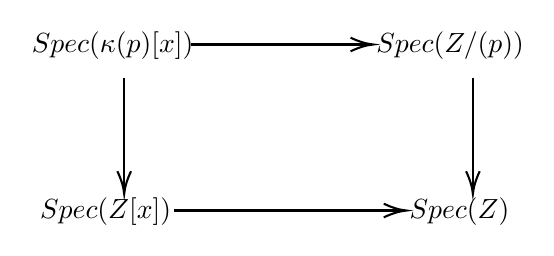
\begin{tikzpicture}[x=0.75pt,y=0.75pt,yscale=-1,xscale=1]
%uncomment if require: \path (0,476); %set diagram left start at 0, and has height of 476

%Straight Lines [id:da4576996492347125] 
\draw    (248,192) -- (334,192) ;
\draw [shift={(336,192)}, rotate = 180] [color={rgb, 255:red, 0; green, 0; blue, 0 }  ][line width=0.75]    (10.93,-3.29) .. controls (6.95,-1.4) and (3.31,-0.3) .. (0,0) .. controls (3.31,0.3) and (6.95,1.4) .. (10.93,3.29)   ;
%Straight Lines [id:da088557734678675] 
\draw    (216,208) -- (216,262) ;
\draw [shift={(216,264)}, rotate = 270] [color={rgb, 255:red, 0; green, 0; blue, 0 }  ][line width=0.75]    (10.93,-3.29) .. controls (6.95,-1.4) and (3.31,-0.3) .. (0,0) .. controls (3.31,0.3) and (6.95,1.4) .. (10.93,3.29)   ;
%Straight Lines [id:da7521559935110449] 
\draw    (384,208) -- (384,262) ;
\draw [shift={(384,264)}, rotate = 270] [color={rgb, 255:red, 0; green, 0; blue, 0 }  ][line width=0.75]    (10.93,-3.29) .. controls (6.95,-1.4) and (3.31,-0.3) .. (0,0) .. controls (3.31,0.3) and (6.95,1.4) .. (10.93,3.29)   ;
%Straight Lines [id:da9763436140563071] 
\draw    (240,272) -- (350,272) ;
\draw [shift={(352,272)}, rotate = 180] [color={rgb, 255:red, 0; green, 0; blue, 0 }  ][line width=0.75]    (10.93,-3.29) .. controls (6.95,-1.4) and (3.31,-0.3) .. (0,0) .. controls (3.31,0.3) and (6.95,1.4) .. (10.93,3.29)   ;

% Text Node
\draw (174,264.4) node [anchor=north west][inner sep=0.75pt]    {$\text{Spec}(\mathbb{Z}[ x])$};
% Text Node
\draw (352,264.4) node [anchor=north west][inner sep=0.75pt]    {$\text{Spec}(\mathbb{Z})$};
% Text Node
\draw (170,184.4) node [anchor=north west][inner sep=0.75pt]    {$\text{Spec}( \kappa ( p)[ x])$};
% Text Node
\draw (336,184.4) node [anchor=north west][inner sep=0.75pt]    {$\text{Spec}(\mathbb{Z} /( p))$};


\end{tikzpicture}
\end{center}
Therefore for $(0)$, the fiber over it is $\mathrm{Spec}(\mathbb{Q}\otimes_{\mathbb{Z}}\mathbb{Z}[x])=\mathrm{Spec}(\mathbb{Q}(x))$, which consists of irreducible polynomials in $\mathbb{Q}[x]$. For $(p)$, on the other hand, the fiber over it is $\mathrm{Spec}(\mathbb{Z}_p[x])$, which is just irreducible polynomials over $\mathbb{Z}_p[x]$ and the zero ideal (corresponds to those in $\mathbb{Z}$).
\end{proof}
\begin{note}\em
We used the language of Algebraic Geometry to characterize $\mathrm{Spec}(\mathbb{Z}[x])$. Indeed one may use only Abstract Algebra to solve this. One may consider a prime ideal $\mathfrak{p}$ intersect with $\mathbb{Z}$, and transform the language of Algebraic Geometry into Abstract Algebra, which is more elementary but with cumbersome details.
\end{note}
\begin{problem}\em
For each $f\in A$, let $X_f$ denote the complement of $V(f)$ in $X=\mathrm{Spec}(A)$. The sets $X_f$ are open. Show that they form a basis of open sets for the Zariski topology, and that \par
(i) $X_f\cap X_g=X_{fg}$;\par
(ii) $X_f=\emptyset$ if and only if $f$ is nilpotent;\par
(iii) $X_f=X$ if and only if $f$ is a unit;\par
(iv) $X_f=X_g$ if and only if $r((f))=r((g))$;\par
(v) $X$ is quasi-compact;\par
(vi) More generally, each $X_f$ is quasi-compact;\par
(vii) An open subset of $X$ is quasi-compact if and only if it is a finite union of sets $X_f$.
\end{problem}
\begin{proof}
Trivially $\emptyset$ and $\mathrm{Spec}(A)\in\{X_f\}_{f\in A}$. The fact that every prime ideal $\mathfrak{p}$ in the intersection of two elements has a neighborhood in $\{X_f\}_{f\in A}$ follows from (i) below.\par
(i) This is trivial once observe that $X_f\cap X_g=(V(f)\cup V(g))^c=(V(fg))^c=X_{fg}$.\par
(ii) Suppose $X_f=\emptyset$, then $V(f)=\mathrm{Spec}(A)$. Hence for all $\mathfrak{p}\in\mathrm{Spec}(A)$ we have $f\subset\mathfrak{p}$, therefore 
$$
f\in \bigcap_{\mathfrak{p} \in \mathrm{Spec}\left( A \right)}{\mathfrak{p}}=\mathfrak{N} .
$$
Therefore $f$ is nilpotent. Conversely, if $f$ is nilpotent, then $f\in\mathfrak{N}$ and hence $f$ lies in every prime ideal of $A$, hence $V(f)=\mathrm{Spec}(A)$.\par
(iii) Suppose $X_f=X$, then $V(f)=\emptyset$. Therefore $f$ does not lie in any prime ideal, which includes maximal ideals. Therefore $f$ is a unit. Conversely if $f$ is a unit, then $V(f)$ is the set of all prime ideals that contain the whole space, which is the null set.\par
(iv) Suppose $X_f=X_g$. We may also suppose that both $f$ and $g$ are ideals. Therefore 
$$
r\left( f \right) =\bigcap{\left\{ \mathfrak{p} \in \mathrm{Spec}\left( A \right) :f\subset \mathfrak{p} \right\}}\subset \bigcap{\left\{ \mathfrak{p} \in \mathrm{Spec}\left( A \right) :g\subset \mathfrak{p} \right\}}=r\left( g \right) .
$$
Therefore $r(f)\subset r(g)$. However the converse inclusion is also true by a symmetric procedure, hence $r(f)=r(g)$. Now for another direction, if $r(f)=r(g)$, then 
$$
\bigcap{\left\{ \mathfrak{p} \in \mathrm{Spec}\left( A \right) :f\subset \mathfrak{p} \right\}}=\bigcap{\left\{ \mathfrak{p} \in \mathrm{Spec}\left( A \right) :g\subset \mathfrak{p} \right\}},
$$
which implies that the prime ideals $\mathfrak{p}$ of $A$ that containing $f$ coincide with those containing $g$, whence $X_f=X_g$.\par
(v) Suppose $\{X_f\}_{f\in I}$ is a cover of $\mathrm{Spec}(A)$. Then 
$$
\bigcup_{f\in I}{X_f}=\bigcup_{f\in I}{\left( V\left( f \right) \right) ^c}=\left( \bigcap_{f\in I}{V\left( f \right)} \right) ^c.
$$
Therefore 
$$
\bigcap_{f\in I}{V\left( f \right)}=\emptyset .
$$
We claim that $1\in I$. Suppose not, then there exists some maximal ideal $\mathfrak{m}$ such that $\mathfrak{m}\in\bigcap_fV(f)$, a contradiction. Hence $1=\sum_{j=1}^na_jf_j$ for a linear combination of a finite many elements in $I$. Hence 
$$
\mathrm{Spec}\left( A \right) =\left( \bigcap_{i=1}^n{V\left( f_i \right)} \right) ^c=\bigcup_{i=1}^n{X_{f_i}}
$$
is a subcover of $\mathrm{Spec}(A)$, whence $\mathrm{Spec}(A)$ is quasi-compact.\par
(vi) Suppose $\{X_{f_i}\}_{i\in I}$ is a cover of $X_f$. Then 
$$
X_f=\bigcup_{i\in I}{\left( X_{f_i}\cap X_f \right)}=\bigcup_{i\in I}{X_{ff_i}}.
$$
To simplify the notations, we shall write $ff_i$ as $f_i$. Now 
$$
X_f=\left( V\left( f \right) \right) ^c=\bigcup_{i\in I}{\left( V\left( f_i \right) \right) ^c}=\left( \bigcap_{i\in I}{V\left( f_i \right)} \right) ^c,
$$
hence 
$$
V\left( f \right) =\bigcap_{i\in I}{V\left( f_i \right)}.
$$
Therefore $r(f)=r(\{f_i\}_{i\in I})$ and hence $f^n=\sum_{j=1}^ma_jf_j$ for a finite many elements in $I$. Therefore 
$$
f^n=\sum_{j=1}^m{a_jf_j}\in \bigcap_{i\in I}{V\left( f_i \right)}=V\left( f \right) .
$$
Note that if $f^n\in\mathfrak{p}$, then $f\in\mathfrak{p}$ since $\mathfrak{p}$ is prime. Hence 
$$
V\left( f \right) \supset \bigcap_{j=1}^m{V\left( f_j \right)}=V\left( \bigcup_{j=1}^m{f_j} \right) .
$$
Hence $\{x_{f_j}\}_{j=1}^m$ is a subcover of $X_f$ and hence $X_f$ is quasi-compact.\par
(vii) If an open set $O$ is a finite union of sets $X_f$, then clearly it is quasi-compact. Now we prove the converse. Since $\{X_f\}_{f\in A}$ is an open basis of $\mathrm{Spec}(A)$, we may choose (maybe infinitely many) $\{X_{f_i}\}_{i\in I}$ to be an open cover of $O$ such that $O=\bigcup_iX_{f_i}$. Since $O$ is quasi-compact, there are finitely many $\{X_{f_j}\}_{j=1}^n$ that forms a subcover. Therefore 
$$
O\subset \bigcup_{j=1}^n{X_{f_j}}\subset \bigcup_{i\in I}{X_{f_i}}=O,
$$
which finished the proof.
\end{proof}
\begin{note}\em
The sets $X_f$ are called \textbf{basic open sets} of $X=\mathrm{Spec}(A)$.
\end{note}
\begin{problem}\em
It is sometimes convenient to denote a prime ideal of $A$ by a letter such as $x$ or $y$ when thinking of it as a point of $X=\mathrm{Spec}(A)$. When thinking of $x$ as a prime ideal of $A$, we denote it by $\mathfrak{p}_x$. Show that \par
(i) The set $\{x\}$ is closed (we say $x$ a closed point) in $\mathrm{Spec}(A)$ if and only if $\mathfrak{p}_x$ is maximal;\par
(ii) $\overline{\{x\}}=V(\mathfrak{p}_x)$;\par
(iii) $y\in\overline{\{x\}}$ if and only if $\mathfrak{p}_x\subset\mathfrak{p}_y$;\par
(iv) $X$ is a $T_0$-space.
\end{problem}
\begin{proof}
(i) Suppose $\{x\}$ is closed. Then the set $V(\mathfrak{p})=\{x\}$ for some $\mathfrak{p}$. This is possible only if $\mathfrak{p}=\mathfrak{p}_x$ is a maximal ideal. Conversely, if $\mathfrak{p}_x$ is a maximal ideal, then $\{x\}=V(\mathfrak{p}_x)$ is closed.\par
(ii) By definition of a closure, we have 
$$
\overline{\left\{ x \right\} }=\bigcap{\left\{ \mathfrak{p} \in \mathrm{Spec}\left( A \right) :\mathfrak{p} _x\in V\left( \mathfrak{p} \right) \right\}}=\bigcap{\left\{ V\left( \mathfrak{p} \right) :\mathfrak{p} \subset \mathfrak{p} _x \right\}}=V\left( \mathfrak{p} _x \right) .
$$\par
(iii) Suppose $y\in\overline{\{x\}}$, then $\mathfrak{p}_y\in V(\mathfrak{p}_x)$ and hence $\mathfrak{p}_x\subset\mathfrak{p}_y$.\par
(iv) Suppose $x$ and $y$ are distinct points in $\mathrm{Spec}(A)$. Then if $y$ lies in every neighborhood of $x$ and vice versa, we have $\mathfrak{p}_x\subset\mathfrak{p}_y\subset\mathfrak{p}_x$, hence $x=y$, a contradiction.
\end{proof}
\begin{problem}\em
A topological space $X$ is said to be \textbf{irreducible} if $X\ne\emptyset$ and if every pair of non-empty open sets in $X$ intersect, or equivalently if every non-empty open set is dense in $X$. Show that $\mathrm{Spec}(A)$ is irreducible if and only if the nilradical of $A$ is a prime ideal.
\end{problem}
\begin{proof}
Suppose $\mathrm{Spec}(A)$ is irreducible, then for arbitrary nonempty two open sets, say $O_1$ and $O_2$, there intersection is nonempty. Since $\{X_f\}_{f\in A}$ is a basis of $\mathrm{Spec}(A)$, we may suppose $O_1=X_f$ and $O_2=X_g$. Therefore $X_f\cap X_g=X_{fg}$ is nonempty. Therefore $f,g\notin\mathfrak{N}$ implies $fg\notin\mathfrak{N}$, whence $\mathfrak{N}$ is a prime ideal. Conversely, if $\mathfrak{N}$ is a prime ideal, then if $fg\in\mathfrak{N}$, we have $f\in\mathfrak{N}$ or $g\in\mathfrak{N}$. Therefore suppose $X_f$ and $X_g$ are two nonempty open set, then $f$ and $g\notin\mathfrak{N}$. This implies $fg\notin\mathfrak{N}$ and hence $X_{fg}$ nonempty.
\end{proof}
\begin{problem}\em
Let $X$ be a topological space.\par
(i) If $Y$ is irreducible subspace of $X$, then the closure $\overline{Y}$ of $Y$ in $X$ is irreducible. \par
(ii) Every irreducible subspace of $X$ is contained in a maximal irreducible subspace. \par
(iii) The maximal irreducible subspaces of $X$ are closed and cover $X$. They are called the \textbf{irreducible components} of $X$. What are the irreducible components of a Hausdorff space?\par
(iv) If $A$ is a ring and $X=\mathrm{Spec}(A)$, then the irreducible components of $X$ are the closed sets $V(\mathfrak{p})$, where $\mathfrak{p}$ is a minimal prime ideal of $A$.
\end{problem}
\begin{proof}
(i) Suppose $U$ and $V$ are open sets in $\overline{Y}$, then $U\cap Y\ne\emptyset$, $V\cap Y\ne\emptyset$. Therefore $U\cap V\cap Y\ne\emptyset$ since $Y$ is irreducible. This implies $U\cap V\ne\emptyset$ and hence $\overline{Y}$ is irreducible.\par
(ii) We proof by Zorn's lemma. Define an order on the set of irreducible subspaces of a space, and suppose $\{X_{\alpha}\}_{\alpha\in A}$ is a chain.  Let $X=\bigcup_{\alpha\in A}X_\alpha$, then by Zorn's lemma it suffices to show that $X$ is irreducible. Suppose $U$ and $V$ are open sets in $X$, then there exists some $X_\alpha$ and $X_\beta$ such that $U\cap X_\alpha\ne\emptyset$, $V\cap X_\beta\ne\emptyset$. Suppose $X_\alpha\subset X_\beta$, then $U\cap X_\beta\ne\emptyset$. Since $X_\beta$ is irreducible, we have $U\cap V\ne\emptyset$ and hence $X$ is irreducible.\par
(iii) Since the closure of an irreducible subspace is irreducible, we have the maximal irreducible subspaces of $X$ are closed. To see $X$ is covered by its maximal irreducible subspaces, suppose $x$ is not contained in any maximal irreducible subspaces. Then since $x$ itself is an irreducible subspace of $X$, we have $x$ maximal.\par
Now for a Hausdorff space $H$, since for any two distinct element in $H$, there exists two open neighborhoods of each point such that does not intersect. Therefore the only irreducible components in $H$ are singletons.\par
(iv) We first show that $V(I)$ is irreducible if and only if $r(I)$ is prime. To see this, suppose $I$ is an ideal of $A$ and $V(I)$ a closed set in $\mathrm{Spec}(A)$. Then there is a correspondence of closed sets generated by ideals that contain $I$ of the space $\mathrm{Spec}(A)$ and $\mathrm{Spec}(A/I)$. Note that $V(I)$ in $\mathrm{Spec}(A)$ corresponds $V(\mathfrak{N})$ in $\mathrm{Spec}(A/I)$, and $V(\mathfrak{N})$ is irreducible if and only if $\mathfrak{N}$ is prime, we have $r(I)$ a prime ideal in $A$. Conversely, suppose $r(I)$ is prime, then $\mathfrak{N}$ is prime in $A/I$. Therefore $V(\mathfrak{N})$ is irreducible in $\mathrm{Spec}(A/I)$ and hence $V(I)$ irreducible in $\mathrm{Spec}(A)$.\par
Now by the preceding discussion we have $V(\mathfrak{p})$ is irreducible when $\mathfrak{p}$ is prime. Therefore it suffices to find the largest $V(\mathfrak{p})$, which is the case when $\mathfrak{p}$ is the minimal prime ideal.
\end{proof}
\begin{problem}\em
Let $\phi$ be a ring homomorphism. Let $X=\mathrm{Spec}(A)$ and $Y=\mathrm{Spec}(B)$. If $\mathfrak{q}\in Y$, then $\phi^{-1}(\mathfrak{q})$ is a prime ideal of $A$, i.e. a point of $X$. Hence $\phi$ induces a mapping $\phi^*:Y\to X$. Show that \par
(i) If $f\in A$ then $\phi^{*-1}(X_f)=Y_{\phi(f)}$, and hence $\phi^*$ is continuous.\par
(ii) If $\mathfrak{a}$ is an ideal of $A$, then $\phi^{*-1}(V(\mathfrak{a}))=V(\mathfrak{a}^e)$.\par
(iii) If $\mathfrak{b}$ is an ideal of $B$, then $\overline{\phi^*(V(\mathfrak{b}))}=V(\mathfrak{b}^c)$.\par
(iv) If $\phi$ is surjective, then $\phi^*$ is a homeomorphism of $Y$ onto the closed subset $V(\mathrm{Ker}\phi)$ of $X$. In particular, $\mathrm{Spec}(A)$ and $\mathrm{Spec}(A/\mathfrak{N})$ are naturally homeomorphic.\par
(v) If $\phi$ is injective, then $\phi^*(Y)$ is dense in $X$. More precisely, $\phi^*(Y)$ is dense in $X$ if and only if $\mathrm{Ker}\phi\subset\mathfrak{N}$.\par
(vi) Let $\psi:B\to C$ be another ring homomorphism. Then $(\psi\circ\phi)^*=\phi^*\circ\psi^*$.\par
(vii) Let $A$ be an integral domain with just one non-zero prime ideal $\mathfrak{p}$, and let $K$ be the field of fractions of $A$. Let $B=(A/\mathfrak{p})\times K$. Define $\phi:A\to B$ by $\phi(x)=(\overline{x},x)$, where $\overline{x}$ is the image of $x$ in $A/\mathfrak{p}$. Show that $\phi^*$ is bijective but not a homeomorphism.
\end{problem}
\begin{proof}
(i) Suppose $\mathfrak{q}\in Y_{\phi(f)}$. Then $\mathfrak{q}\subset\phi(f)$ and hence $\phi^{-1}(\mathfrak{q})\subset f$. This implies $\phi^{-1}(\mathfrak{q})\in X_f$ and hence $\mathfrak{q}\in\phi^{*-1}(X_f)$. Conversely, suppose $\mathfrak{q}\in\phi^{*-1}(X_f)$. Then $\phi^{-1}(\mathfrak{q})\subset f$ and hence $\mathfrak{q}\subset\phi(f)$. This implies $\mathfrak{q}\in Y_{\phi(f)}$. \par
(ii) Suppose $\mathfrak{q}\in V(\mathfrak{a}^e)$. Then $\mathfrak{a}^e\subset\mathfrak{q}$ and hence $\mathfrak{a}\subset\phi^{-1}(\mathfrak{q})$. Hence $\mathfrak{q}\in\phi^{*-1}(\mathfrak{a})$. Conversely, suppose $\mathfrak{q}\in\phi^{*-1}(V(\mathfrak{a}))$, then $\mathfrak{a}\subset\phi^{-1}(\mathfrak{q})$ and hence $\mathfrak{a}^e\subset\mathfrak{q}$. This implies $\mathfrak{q}\in V(\mathfrak{a}^e)$ and hence $\phi^{*-1}(V(\mathfrak{a}))\subset V(\mathfrak{a}^e)$.\par
(iii) We first prove a lemma. Suppose $I$ is an ideal of $A$, then $V(I)=V(r(I))$. Since $I\subset r(I)$, trivially we have $V(r(I))\subset V(I)$. Conversely, suppose $x\in V(I)$, then $I\subset x$. Now suppose $f\in r(I)$, then $f^n\in I$ for some $n$. Since $\mathfrak{p}$ is prime, we have $f\in\mathfrak{p}$ and hence $r(I)\subset\mathfrak{p}$.\par
Now suppose $\mathfrak{p}\in V(\mathfrak{b}^c)$. Then $\mathfrak{b}^c\subset\mathfrak{p}$ and hence $\mathfrak{b}\subset\phi(\mathfrak{p})$. Therefore $\mathfrak{p}\in\phi^*(V(\mathfrak{b}))$. Since $V(\mathfrak{b}^c)$ is closed, we may take a closure over $\phi^*(V(\mathfrak{b}))$ and the inclusion relation does not change. Conversely, since $\overline{\phi^*(V(\mathfrak{b}))}$ is closed, there exists some $\mathfrak{a}$ such that $\overline{\phi^*(V(\mathfrak{b}))}=V(\mathfrak{a})$. Therefore 
$$
V\left( \mathfrak{a} ^e \right) =\phi ^{*-1}V\left( \mathfrak{a} \right) =\phi ^{*-1}\overline{\phi ^*\left( V\left( \mathfrak{b} \right) \right) }\supset V\left( \mathfrak{b} \right) ,
$$
hence $\mathfrak{a} ^e\subset \sqrt{\mathfrak{b}}$. Therefore by the lemma we have 
$$
\overline{\phi ^*\left( V\left( \mathfrak{b} \right) \right) }=V\left( \mathfrak{a} \right) \supset V\left( r\left( \mathfrak{b} ^c \right) \right) =V\left( \mathfrak{b} ^c \right) ,
$$
which finished the proof.\par
(iv) We first claim that if $\phi:A\to B$ is an isomorphism, then $\phi^*$ is a homeomorphism. By (i) we have $\phi^*$ is continuous. Since $\phi$ is an isomorphism, there exists some $\psi$ that is the inverse map of $\phi$. Therefore $\psi^*$ is the inverse of $\phi^*$ and hence $\phi^*$ a homeomorphism between $\mathrm{Spec}(B)$ and $\mathrm{Spec}(A)$.\par
Now suppose $\phi$ is a monomorphism. Since $A/\mathrm{Ker}\phi\cong B$, we have $\phi^*$ induces a homeomorphism between $\mathrm{Spec}(B)$ and $\mathrm{Spec}(A/\mathrm{Ker}\phi)$. Now it suffices to show that there is a homeomorphism between elements of $\mathrm{Spec}(A/\mathrm{Ker}\phi)$ and $V(\mathrm{Ker}\phi)$. Note that there is a one-to-one correspondence given by the canonical projection $A\to A/\mathrm{Ker}\phi$, it suffices to show that $\pi^*(V(\mathfrak{a}+\mathrm{Ker}\phi))=V(\mathfrak{a})$, where $\mathfrak{a}$ is an ideal of $A$ that contains $\mathrm{Ker}\phi$. This follows from an easy inclusion discussion. (See the diagram below)
\begin{center}


\tikzset{every picture/.style={line width=0.75pt}} %set default line width to 0.75pt        

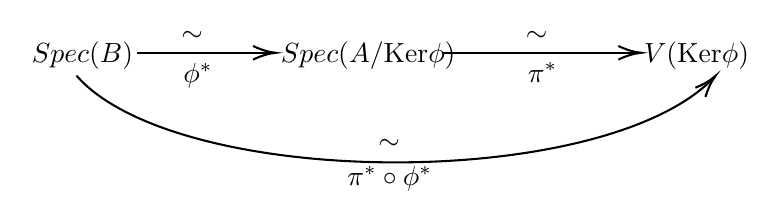
\begin{tikzpicture}[x=0.75pt,y=0.75pt,yscale=-1,xscale=1]
%uncomment if require: \path (0,476); %set diagram left start at 0, and has height of 476

%Straight Lines [id:da3464817478310078] 
\draw    (221,189) -- (286,189) ;
\draw [shift={(288,189)}, rotate = 180] [color={rgb, 255:red, 0; green, 0; blue, 0 }  ][line width=0.75]    (10.93,-3.29) .. controls (6.95,-1.4) and (3.31,-0.3) .. (0,0) .. controls (3.31,0.3) and (6.95,1.4) .. (10.93,3.29)   ;
%Straight Lines [id:da599396113938103] 
\draw    (368,189) -- (462,189) ;
\draw [shift={(464,189)}, rotate = 180] [color={rgb, 255:red, 0; green, 0; blue, 0 }  ][line width=0.75]    (10.93,-3.29) .. controls (6.95,-1.4) and (3.31,-0.3) .. (0,0) .. controls (3.31,0.3) and (6.95,1.4) .. (10.93,3.29)   ;
%Curve Lines [id:da51919648788218] 
\draw    (192,200) .. controls (240.16,254.86) and (446.32,256.32) .. (499.21,200.84) ;
\draw [shift={(500,200)}, rotate = 132.49] [color={rgb, 255:red, 0; green, 0; blue, 0 }  ][line width=0.75]    (10.93,-3.29) .. controls (6.95,-1.4) and (3.31,-0.3) .. (0,0) .. controls (3.31,0.3) and (6.95,1.4) .. (10.93,3.29)   ;

% Text Node
\draw (169,182.4) node [anchor=north west][inner sep=0.75pt]    {$\text{Spec}( B)$};
% Text Node
\draw (241,177.4) node [anchor=north west][inner sep=0.75pt]    {$\sim $};
% Text Node
\draw (242,192.4) node [anchor=north west][inner sep=0.75pt]    {$\phi ^{*}$};
% Text Node
\draw (289,182.4) node [anchor=north west][inner sep=0.75pt]    {$\text{Spec}( A/\mathrm{Ker} \phi )$};
% Text Node
\draw (407,177.4) node [anchor=north west][inner sep=0.75pt]    {$\sim $};
% Text Node
\draw (408,192.4) node [anchor=north west][inner sep=0.75pt]    {$\pi ^{*}$};
% Text Node
\draw (464,182.4) node [anchor=north west][inner sep=0.75pt]    {$V(\mathrm{Ker} \phi )$};
% Text Node
\draw (336,229.4) node [anchor=north west][inner sep=0.75pt]    {$\sim $};
% Text Node
\draw (321,242.4) node [anchor=north west][inner sep=0.75pt]    {$\pi ^{*} \circ \phi ^{*}$};


\end{tikzpicture}
\end{center}
Note that $V(\mathfrak{N})=\mathrm{Spec}(A)$, hence there is a natural homeomorphism between $\mathrm{Spec}(A)$ and $\mathrm{Spec}(A/\mathfrak{N})$.
\par
(v) Suppose $\phi^*$ is dense in $X$, then 
$$
X=\overline{\phi ^*\left( Y \right) }=\overline{\phi ^*\left( V\left( 0 \right) \right) }=V\left( 0^c \right) =V\left( \mathrm{Ker}\phi \right) .
$$
Therefore $\mathrm{Ker}\phi\subset\mathfrak{p}$ for all $\mathfrak{p}\in\mathrm{Spec}(A)$, which implies $\mathrm{Ker}\phi\subset\mathfrak{N}$. Conversely, if $\mathrm{Ker}\phi\subset\mathfrak{N}$, then 
$$
\overline{\phi ^*\left( Y \right) }=\overline{\phi ^*\left( V\left( 0 \right) \right) }=V\left( 0^c \right) =V\left( \mathrm{Ker}\phi \right) =X,
$$
which implies $\phi^*(Y)$ is dense in $X$.\par
(vi) Note that 
$$
a\in \left( \psi \circ \phi \right) ^*\left( X \right) \Longleftrightarrow \left( \psi \circ \phi \right) \left( a \right) \in X\Longleftrightarrow \phi \left( a \right) \in \psi ^*\left( X \right) \Longleftrightarrow a\in \left( \phi ^*\circ \psi ^* \right) \left( X \right) .
$$\par
(vii) We first show that $\phi^*$ is bijective. To do this, we need to characterize the prime ideals in $B$. First note that the ideals of $A$ are $0$ and $\mathfrak{p}$, whence the ideals of $A/\mathfrak{p}$ are $\overline{0}$ and $\overline{1}$. Since $K$ is a field, the only ideals of it is $0$ and $K$. Therefore there are four ideals of $B$: 
$$
\overline{0}\times 0,\hspace{0.5cm}\overline{0}\times K,\hspace{0.5cm}\overline{1}\times 0,\hspace{0.5cm}\overline{1}\times K.
$$
Verify by definition we obtain 
$$
\mathrm{Spec}\left( B \right) =\left\{ \overline{0}\times K,\overline{1}\times 0 \right\} =\left\{ \mathfrak{q} _1,\mathfrak{q} _2 \right\} .
$$
By definition we have $\phi ^{-1}\left( \mathfrak{q} _1 \right) =\mathfrak{p} ,\phi ^{-1}\left( \mathfrak{q} _2 \right) =0$, hence $\phi$ is a bijection. However there are three distinct closed sets on $\mathrm{Spec}(A)$, but $\mathrm{Spec}(B)$ is equipped with the discrete topology. Therefore $\mathrm{Spec}(A)\not\simeq\mathrm{Spec}(B)$ and hence $\phi^*$ is not a homeomorphism.
\end{proof}
\begin{problem}\em
Let $A=\oplus_{i=1}^nA_i$ be the direct product of rings $A_i$. Show that $\mathrm{Spec}(A)$ is the disjoint union of open (and closed) subspaces $X_i$, where $X_i$ is canonically homeomorphic with $\mathrm{Spec}(A_i)$.\par
Conversely, let $A$ be a ring. Show that the following statements are equivalent:\par
(i) $X=\mathrm{Spec}(A)$ is disconnected.\par
(ii) $A\cong A_1\times A_2$ where neither of the rings $A_1$ and $A_2$ is the zero ring.\par
(iii) $A$ contains an idempotent $0$, $1$.\par
In particular, the spectrum of a local ring is always connected.
\end{problem}
\begin{proof}
We first prove the first assertion. Consider the canonical projections $\pi _i:A=\bigoplus_{i=1}^n{A_i}\rightarrow A_i$ whose kernel is $\bigoplus_{j\ne i}A_j$. Therefore by Exercise 7.7(iv) we have 
$$
\mathrm{Spec}\left( A/\bigoplus_{j\ne i}{A_j} \right) \simeq V\left( \bigoplus_{j\ne i}{A_j} \right) 
$$
for all $j$. Now we consider $\left\{V\left(\bigoplus_{j\ne i}A_j\right)\right\}_{j=1}^n$. We first show that it is a cover of $\mathrm{Spec}(A)$, which suffices to note that 
$$
\bigcup_{j=1}^n{V\left( \bigoplus_{j\ne i}{A_j} \right)}=V\left( \bigcap_{j=1}^n{\bigoplus_{j\ne i}{A_j}} \right) =V\left( 0 \right) =\mathrm{Spec}\left( A \right) .
$$
Now for the disjoint property, we note that 
$$
V\left( \bigoplus_{j\ne i_1}{A_j} \right) \cap V\left( \bigoplus_{j\ne i_2}{A_j} \right) =V\left( \bigoplus_{j\ne i_1}{A_j}\cup \bigoplus_{j\ne i_2}{A_j} \right) =V\left( \mathrm{Spec}\left( A \right) \right) =\emptyset .
$$
Therefore 
$$
\mathrm{Spec}\left( A \right) =\bigsqcup_{j=1}^n{V\left( \bigoplus_{j\ne i}{A_j} \right)}\simeq \bigsqcup_{j=1}^n{\mathrm{Spec}\left( A_i \right)},
$$
which finished the proof.\par
For the particular case, we proof that in a local ring the only idempotent elements are $0$ and $1$. Suppose $e^2=e\ne 0,1$ in a local ring $A$. Then $e$ is not a unit, and hence contained in some maximal ideals $\mathfrak{m}$. Note that the only maximal ideal in $A$ is the Jacobson radical $\mathfrak{R}$, hence $1-e$ is a unit, contradiction.
\end{proof}
\begin{problem}\em
Let $A$ be a Boolean ring, and let $X=\mathrm{Spec}(A)$.\par
(i) For each $f\in A$, the set $X_f$ is both open and closed in $X$.\par
(ii) Let $f_1,\cdots,f_n\in A$. Show that $X_{f_1}\cup\cdots\cup X_{f_n}=X_f$ for some $f\in A$.\par
(iii) The sets $X_f$ are the only subsets of $X$ which are both open and closed.\par
(iv) $X$ is a compact Hausdorff space.
\end{problem}
\begin{proof}
(i) $X_f$ is trivially open in $X$. We now show that $X_f$ is closed. Indeed, we observe that $X=X_f\sqcup X_{1-f}$, therefore $X_f=V(1-f)$. To show this, we first show that $X_f$ and $X_{1-f}$ are disjoint. It suffices to notice that 
$$
X_f\cap X_{1-f}=X_{f\left( 1-f \right)}=X_0=\emptyset .
$$
To show that $X=X_f\cup X_{1-f}$, we notice that 
$$
X_f\cup X_{1-f}=\left( V\left( f \right) \cap V\left( 1-f \right) \right) ^c=X_{\left( f \right) \cup \left( 1-f \right)}=X_{\left( 1 \right)}=\mathrm{Spec}\left( A \right) .
$$
Hence $X_f=V(1-f)$ is closed.\par
(ii) We first show that in a Boolean ring, every finitely generated ideal is principal. We show this by induction. For $n=1$, trivial. Now suppose this is true for all $k\le n$. Suppose $(x_1,\cdots,x_n,y)$ is an ideal, then there exists some $x$ such that $(x)=(x_1,\cdots,x_n)$. Note that $(x,y)=(x+y-xy)$, we finished the proof. Now notice that 
$$
\bigcup_{i=1}^n{X_{f_i}}=\left( \bigcap_{i=1}^n{V\left( f_i \right)} \right) ^c=\left( V\left( \sum_{i=1}^n{\left( f_i \right)} \right) \right) ^c=X_{\left( f_1,\cdots ,f_n \right)}=X_f
$$
for some $f\in A$, where the last equality follows from the preceding remarks.\par
(iii) Suppose $Y$ is an open set in $X$. Then since $\{X_f\}_{f\in A}$ is an open basis of $X$, we may suppose that $Y=\bigcup_{i\in I}X_{f_i}$. If $Y$ is also closed, then $Y$ is quasi-compact in $X$. Therefore 
$$
Y=\bigcup_{i\in I}{X_{f_i}}=\bigcup_{j=1}^n{X_{f_j}}=X_f
$$
for some $f$ and hence $Y=X_f$.\par
(iv) We have shown that $X$ is quasi-compact. Now it suffices to show that $X$ is Hausdorff. Suppose $x,y\in X$ and $x\ne y$. We show that there exists some $f\in A$ such that $x\in X_f$ and $y\in X_{1-f}$, which are two disjoint open sets. Note that $x\in X_f$ implies $f\notin\mathfrak{p}_x$ and $y\in X_{1-f}$ implies $1-f\notin\mathfrak{p}_y$, which is $f\in\mathfrak{p}_y$. If for all $f\in A$ the two statement cannot be true at the same time, we have $\mathfrak{p}_x\subset\mathfrak{p}_y$. However in a Boolean ring, every prime ideal is maximal, therefore $\mathfrak{p}_x=\mathfrak{p}_y$ and hence $x=y$, a contradiction!
\end{proof}
\begin{problem}\em
Let $L$ be a lattice, in which the sup and inf of two elements $a$, $b$ are denoted by $a\vee b$ and $a\wedge b$ respectively. $L$ is a \textbf{Boolean lattice} or (\textbf{Boolean algebra}) if \par
(a) $L$ has a least element and a greatest element (denoted by $0$, $1$ respectively);\par
(b) Each of $\vee$, $\wedge$ in distributive over another;\par
(c) Each $a\in L$ has a unique "complement" $a^\prime\in L$ such that $a\vee a^\prime=1$ and $a\wedge a^\prime=0$.\par
For example, the set of all subsets of a set, ordered by inclusion, is a Boolean lattice.\par
Let $L$ be a Boolean lattice. Define additive and multiplication in $L$ by the rules 
$$
a+b=\left( a\land b^{\prime} \right) \lor \left( a^{\prime}\land b \right) ,\hspace{0.5cm}ab=a\land b.
$$
Verify that in this way $L$ becomes a Boolean ring, say $A(L)$.\par
Conversely, starting from a Boolean ring $A$, define an ordering on $A$ as follows: $a\le b$ means that $a=ab$. Show that, which respect to this ordering, $A$ is a Boolean lattice. In this way we obtain a one-to-one correspondence between (isomorphism classes of) Boolean rings and (isomorphism classes of) Boolean lattices.
\end{problem}
\begin{proof}
This exercise is proved via boring definition checking. We shall omit the easy but annoying details.
\end{proof}
\begin{problem}\em
From the last two exercises deduce \textbf{Stone's Theorem}, that every Boolean lattice is isomorphic to the lattice to open-and-closed subsets of some compact-Hausdorff topological spaces.
\end{problem}
\begin{proof}
Let $L$ be a Boolean algebra, and $A$ the corresponding Boolean ring. Therefore $\mathrm{Spec}(A)$ is a compact Hausdorff space. Let $B$ be the algebra of simultaneously open and closed sets in $X$. By the definition of open and closed, it is closed under binary union and intersection, so it is a sublattice of the power set $\mathcal{P}(\mathrm{Spec}(A)),\subset$ under inclusion. By the definition of a topology, $\emptyset$, $\mathrm{Spec}(A)\in B$. By set algebra, $\cup$ and $\cap$ each distribute over the other. The complement $V$ of an open and closed set $U$ is open and closed, and is the unique $V\subset\mathcal{P}(\mathrm{Spec}(A))$ with $U\cup V=\mathrm{Spec}(A)$ and $U\cap V=\emptyset$. Thus $B$ is a Boolean algebra.\par
Now note that $B$ is the set of $X_f$ for $f\in A$, define the correspondence $\phi:L\to B$ by $f\mapsto X_f$, then it is routine to check $\phi$ is an isomorphism, which finished the proof.
\end{proof}
\begin{problem}\em
Let $A$ be a ring. The subspace of $\mathrm{Spec}(A)$ consisting of the maximal ideals of $A$, with the induced topology, is called the \textbf{maximum spectrum} of $A$ and is denoted by $\mathrm{Max}(A)$. For arbitrary commutative rings it does not have the nice functorial properties of $\mathrm{Spec}(A)$, since the inverse under a ring homomorphism of a maximal ideal need not be maximal.\par
Let $X$ be a compact Hausdorff space and let $C(X)$ denote the ring of all real-valued continuous functions on $X$. For each $x\in X$, let $\mathfrak{m}_x$ be the set of all $f\in C(X)$ such that $f(x)=0$. The ideal $\mathfrak{m}_x$ is maximal, because it is the kernel of the (surjective) homomorphism $C(X)\to\mathbb{R}$ which takes $f$ to $f(x)$. If $\widetilde{X}=\mathrm{Max}(C(X))$, we have therefore defined a mapping $\mu:X\to\widetilde{X}$, namely $x\mapsto\widetilde{x}$.\par
We shall show that $\mu$ is a homeomorphism of $X$ onto $\widetilde{X}$.\par
(i) Let $\mathfrak{m}$ be any maximal ideal of $C(X)$, and let $V=V(\mathfrak{m})$ be the set of common zeros of the functions in $\mathfrak{m}$, that is, 
$$V(\mathfrak{m})=\{x\in X:f(x)=0\ \text{for all}\ f\in\mathfrak{m}\}.$$
Show that $V$ is nonempty, and $\mu$ is surjective.\par
(ii) Show by Urysorn's lemma that $\mu$ is injective.\par
(iii) Let $f\in C(X)$; let 
$$U_f=\{x\in X:f(x)\ne 0\}$$
and let 
$$\widetilde{U_f}=\{\mathfrak{m}\in\widetilde{X}:f\notin\mathfrak{m}\}.$$
Show that $\mu(U_f)=\widetilde{U_f}$. The open sets $U_f$ [resp. $\widetilde{U_f}$] form a basis of the topology of $X$ [resp. $\widetilde{X}$] and therefore $\mu$ is a homeomorphism.\par
Thus $X$ can be reconstructed from the ring of functions $C(X)$.
\end{problem}
\begin{proof}
(i) We first show that $V$ is nonempty. Suppose $V$ is empty, then for each $x\in X$, there exists some $f_x$ such that $f_x(x)\ne 0$. Therefore there exists a neighborhood of $x$ such that $f_x(U_x)\ne 0$ since $f\in C(X)$. Note that $X$ is compact, therefore there exists a finite open subcover $\{U_i\}_{i=1}^n$ such that $f_i(U_i)\ne 0$ for some $f_i\in C(X)$. Now define $f=\sum_{i=1}^nf_i$, therefore $f\ne 0$. Hence $f\in\mathfrak{m}$ implies $\mathfrak{m}=C(X)$, a contradiction!\par
Now we show that $\mu$ is surjective. Suppose $x\in X$. We first show that $x\in V(\mathfrak{m})$ for some $\mathfrak{m}$. Since there exists some $f\in C(X)$ such that $f(x)=0$, $f$ is not a unit. Therefore $f$ is contained in some maximal ideals $\mathfrak{m}$. Therefore we may suppose $x\in V(\mathfrak{m})$ for some $\mathfrak{m}$. Then $\mathfrak{m}\subset\mathfrak{m}_x$, hence $\mathfrak{m}=\mathfrak{m}_x$ since $\mathfrak{m}$ is maximal.\par
(ii) Suppose $x\ne y$. Since $X$ is a compact Hausdorff space, we may apply Urysorn's lemma to obtain two functions $f_x$ and $f_y$ such that $f_x(x)=f_y(y)=0$ and $f_x(y),f_y(x)\ne 0$. Then $f_y\notin\mathfrak{m}_x$ and $f_x\notin\mathfrak{m}_y$, but $f_x\in\mathfrak{m}_x$ and $f_y\in\mathfrak{m}_y$. This implies $\mathfrak{m}_x\ne\mathfrak{m}_y$ and hence $\mu$ is injective.\par
(iii) We first show that $\mu(U_f)=\widetilde{U_f}$. It suffices to note that 
$$
x\in U_f\Longleftrightarrow f\left( x \right) \ne 0\Longleftrightarrow f\notin \mathfrak{m} _x\Longleftrightarrow \mathfrak{m} _x\in \widetilde{U_f}.
$$
Now we show $\{U_f\}$ form a basis of $X$. Clearly $U_f$ are open. Now suppose $W$ is an open set and $x\in W$, it suffices to show that there exists some $f\in C(X)$ such that $x\in U_f\subset W$. We again apply Urysorn's lemma. Since $W$ is open, we have $X-W$ closed. Therefore there exists some $f\in C(X)$ such that $f(X-W)=0$ and $f(x)=1$. Therefore $x\in U_f\subset W$, finishing the proof.\par
The condition for $\widetilde{X}$ and $\{\widetilde{U_f}\}$ are similar and we skip the proof.
\end{proof}
\begin{center}
\begin{large}
    \textbf{Affine Algebraic Varieties}
\end{large}
\end{center}
\begin{problem}\em
Let $k$ be an algebraic closed field, and let $f_\alpha(t_1,\cdots,t_n)=0$ be a set of polynomial equations in $n$ variables with coefficients in $k$. The set $X$ of all points $x=(x_1,\cdots,x_n)\in k^n$ which satisfy these equations is an \textbf{affine algebraic variety}.\par
Consider the set of all polynomials $g\in k[t_1,\cdots,t_n]$ with the property that $g(x)=0$ for all $x\in X$. This set is an ideal $I(X)$ in the polynomial ring, and is called the \textbf{ideal of the variety $X$}. The quotient ring 
$$P(X)=k[t_1,\cdots,t_n]/I(X)$$
is the ring of polynomial functions on $X$, because two polynomials $g$, $h$ define the same polynomial equation on $X$ if and only if $g-h$ vanishes at every point of $X$, that is, if and only if $g-h\in I(X)$.\par
Let $\xi_i$ be the image of $t_i$ in $P(X)$. The $\xi_i$ $(1\le i\le n)$ are the \textbf{coordinate functions} on $X$: if $x\in X$, then $\xi_i(x)$ is the $i$th coordinate of $x$. $P(X)$ us generated as a $k$-algebra by the coordinate functions, and is called the \textbf{coordinate ring} (or \textbf{affine algebra}) of $X$.\par
As in Exercise 7.12, for each $x\in X$ let $\mathfrak{m}_x$ be the ideal of all $f\in P(X)$ such that $f(x)=0$. It is a maximal ideal of $P(X)$. Hence if $\widetilde{X}=\mathrm{Max}(P(X))$, we have defined a mapping $\mu:X\to\widetilde{X}$, namely $x\mapsto\mathfrak{m}_x$.\par
Show that $\mu$ is both injective and bijective. This is one form of \textbf{Hilbert's Nullstellensatz}.
\end{problem}
\begin{proof}
We only show that $\mu$ is injective. The surjective part will be dealt with when introducing Norther rings.\par
Suppose $x\ne y$, then $x_i\ne y_i$ for some $i$. Consider the coordinate function $\xi_i$, we have $\xi_i-x_i\in\mathfrak{m}_x$, however $\xi_i-x_i\notin\mathfrak{m}_y$. This implies $\mathfrak{m}_x\ne\mathfrak{m}_y$ and hence $\mu$ is injective.
\end{proof}
\begin{problem}\em
Let $f_1,\cdots,f_m$ be elements of $k[t_1,\cdots,t_n]$. They determine a polynomial mapping $\phi:k^n\to k^m$: if $x\in k^n$, the coordinates of $\phi(x)$ are $f_1(x),\cdots,f_m(x)$.\par
Let $X$ and $Y$ be affine algebraic varieties in $k^n$, $k^m$ respectively. A mapping $\phi:X\to Y$ is said to be \textbf{regular} if $\phi$ is the restriction to $X$ of a polynomial mapping from $k^n$ to $k^m$.\par
If $\eta$ is a polynomial function on $Y$, then $\eta\circ\phi$ is a polynomial function on $X$. Hence $\phi$ induces a $k$-algebra homomorphism $\phi^\sharp:P(Y)\to P(X)$, given by $\eta\mapsto\eta\circ\phi$. Show that in this way we obtain a one-to-one correspondence between the regular mappings $X\to Y$ and the $k$-algebra homomorphisms $P(Y)\to P(X)$.
\end{problem}
\begin{proof}
We first show that $\phi^\sharp$ is a homomorphism. Suppose $r\in k$ and $f,g\in P(Y)$. Then we have 
$$
\phi ^{\sharp}\left( rf \right) =rf\circ \phi =r\left( f\circ \phi \right) =r\phi ^{\sharp}\left( f \right) ,
$$
$$
\phi ^{\sharp}\left( f+g \right) =\left( f+g \right) \circ \phi =f\circ \phi +g\circ \phi =\phi ^{\sharp}\left( f \right) +\phi ^{\sharp}\left( g \right) ,
$$
and 
$$
\phi ^{\sharp}\left( fg \right) =fg\circ \phi =\left( f\circ \phi \right) \left( g\circ \phi \right) =\phi ^{\sharp}\left( f \right) \phi ^{\sharp}\left( g \right) .
$$
Therefore $\phi^\sharp$ is a homomorphism.\par
Now we show the correspondence is injective. Suppose $\phi^\sharp=\psi^\sharp$. It suffices to show that $\phi=\psi$. To to this, suppose $\phi_i:k^n\to k$ is the $i$-th coordinate of $\phi$, and similarly define $\psi$. Observe that 
$$
\phi _i=\xi _i\circ \phi =\phi ^{\sharp}\left( \xi _i \right) =\psi ^{\sharp}\left( \xi _i \right) =\xi _i\circ \psi =\psi _i,
$$
we have $\phi_i=\psi_i$ for all $i$, hence $\phi=\psi$.\par
Now we show that $\phi^\sharp$ is surjective. Let $\lambda\in\mathrm{Hom}_k(P(Y),P(X))$. It suffices to find some $\phi\in\mathrm{Hom}(X,Y)$ such that $\phi^\sharp=\lambda$. Define $\kappa=\lambda\circ\pi:k[t_1,\cdots,t_m]\to P(X)$, where $\pi:k[t_1,\cdots,t_m]\to P(Y)$ is the canonical projection, since $P(Y)$ is the quotient ring $k[t_1,\cdots,t_m]/I(Y)$. Then $\phi_i=\lambda\circ\pi_i$ is a regular function, since its preimage lies in $k[t_1,\cdots,t_m]$ and maps to $P(X)=k[t_1,\cdots,t_n]/I(X)$. Now define $\phi$ with coordinates $\phi_i$, $1\le i\le m$. Then 
$$
\lambda \circ \pi \left( \eta \right) =\eta \left( \kappa \left( t_1 \right) ,\cdots ,\kappa \left( t_m \right) \right) =\eta \left( \phi _1\cdots ,\phi _m \right) =\eta \circ \phi =\phi ^{\sharp}\left( \eta \right) .
$$
Now it suffices to show that for all $\eta^\prime=\eta+I(X)$, $\eta\circ\phi=\eta^\prime\circ\phi$. Note that this is equivalent to say that for all $\psi\in I(Y)$, we have $\psi\circ\phi=0$, and 
$$
\psi \circ \phi =\psi \left( \phi _1\cdots ,\phi _m \right) =\psi \left( \kappa \left( t_1 \right) ,\cdots ,\kappa \left( t_m \right) \right) =\kappa \left( \psi \right) =\lambda \circ \pi \left( \psi \right) =\lambda \left( 0 \right) =0,
$$
hence $\lambda=\phi^\sharp$ and the correspondence is injective.\par
Eventually, suppose given $\phi:X\to Y$ and $\psi:Y\to Z$, we have 
$$
\left( \psi \circ \phi \right) ^{\sharp}\left( \zeta \right) =\zeta \circ \psi \circ \phi =\phi ^{\sharp}\left( \zeta \circ \psi \right) =\left( \phi ^{\sharp}\circ \psi ^{\sharp} \right) \left( \zeta \right) ,
$$
hence the coordinate rig is a contravariant functor from the category of affine algebraic varieties and regular maps to the category of finitely generated $k$-algebras and $k$-algebra homomorphisms.
\end{proof}
\begin{center}
\begin{large}
    \textbf{Miscellaneous Problems}
\end{large}
\end{center}
\begin{problem}\em
A ring $A$ is such that every ideal not contained in the nilradical contains a nonzero idempotent. Prove that the nilradical and Jacobson radical of $A$ are equal.
\end{problem}
\begin{proof}
Since every maximal ideal is prime, trivially we have $\mathfrak{N}\subset\mathfrak{R}$. To prove the inverse inclusion, suppose $a\notin\mathfrak{N}$. Therefore $(a)\notin\mathfrak{N}$ and hence $ax=e$ for some $x\in A$, where $e$ is an idempotent. Since $(1-e)e=0$, $1-e=1-ax$ is not a unit. Therefore $a\notin\mathfrak{R}$ and hence $\mathfrak{N}=\mathfrak{R}$.
\end{proof}
\begin{problem}\em
Let $A$ be a ring in which every element $x$ satisfies $x^n=x$ for some $n>1$ depending on $x$. Show that every prime ideal in $A$ is maximal.
\end{problem}
\begin{proof}
Let $\mathfrak{p}$ be a prime ideal of $A$. Consider $A/\mathfrak{p}$, which is an integral domain. Since $x^n=x$, we have $\overline{x}^n=\overline{x}$, where $\overline{x}$ denote the equivalent class of $x$ in $A/\mathfrak{p}$. Since $A/\mathfrak{p}$ is an integral domain, we may cancel $\overline{x}$ to obtain $\overline{x}^{-1}=\overline{x}^{n-2}$ for all $\overline{x}\in A/\mathfrak{p}$, therefore $A/\mathfrak{p}$ is a field. This implies $\mathfrak{p}$ a maximal ideal.
\end{proof}
\begin{problem}\em
Let $\mathfrak{a}$ be an ideal $\ne (1)$ in a ring $A$. Show that $\mathfrak{a}=r(\mathfrak{a})$ if and only if $\mathfrak{a}$ is the intersection of prime ideals.
\end{problem}
\begin{proof}
Suppose $\mathfrak{a}=r(\mathfrak{a})$. Then 
$$
\mathfrak{a} =r\left( \mathfrak{a} \right) =\bigcap{\left\{ \mathfrak{p} \in \mathrm{Spec}\left( A \right) :\mathfrak{a} \subset \mathfrak{p} \right\}}
$$
is an intersection of some prime ideals. Conversely, $\mathfrak{a}=\bigcap_i\mathfrak{p}_i$ for some $i$, then $x^n\in\mathfrak{a}$ implies $x^n\in\bigcap_i\mathfrak{p}_i$, hence $x\in\bigcap_i\mathfrak{p}_i=\mathfrak{a}$. This implies $\mathfrak{a}=r(\mathfrak{a})$.
\end{proof}
\begin{problem}\em
Let $A$ be a ring, $\mathfrak{N}$ its nilradical. Show that the following are equivalent: \par
(i) $A$ has exactly one prime ideal;\par
(ii) Every element of $A$ is either a unit or nilpotent;\par
(iii) $A/\mathfrak{N}$ is a field.
\end{problem}
\begin{proof}
(i)$\Rightarrow$(ii): Suppose $a\in A$. Then there are two conditions: $a\in\mathfrak{N}$ and $a\notin\mathfrak{N}$. If $a\in\mathfrak{N}$, then $a$ is nilradical by the definition of $\mathfrak{N}$. Otherwise $0\ne\overline{a}\in A/\mathfrak{N}$ is an integral domain, hence $a$ is a unit.\par
(ii)$\Rightarrow$(iii): If $a\in A$ is nilpotent, then $a\in\mathfrak{N}$ and hence $\overline{a}=\overline{0}$. Otherwise $a$ is a unit, hence $\overline{a}\in A/\mathfrak{N}$ has an inverse, this implies $A/\mathfrak{N}$ a field.\par
(iii)$\Rightarrow$(i): Since $A/\mathfrak{N}$ is a field, then $\mathfrak{N}$ is a maximal ideal. Now if 
$$
\mathfrak{N} =\bigcap_{\mathfrak{p} \in \mathrm{Spec}\left( A \right)}{\mathfrak{p}},
$$
we have every $\mathfrak{p}\in\mathrm{Spec}(A)$ coincide, i.e. there is only one prime ideal of $A$.
\end{proof}
\subsection{Further Topics on Modules}
One of the things which distinguishes the modern approach to Commutative Algebra is the greater emphasis on modules, rather than just on ideals. The extra "elbow-room" that this gives makes for greater clarity and simplicity. For instance, an ideal $\mathfrak{a}$ and its quotient ring $A/\mathfrak{a}$ are both examples of modules and so, to a certain extent, can be treated on an equal footing. In this section we discuss modules and tensor products further.
\begin{center}
\begin{large}
    \textbf{Finite Generated Modules}
\end{large}
\end{center}
A \textbf{free} module is one which is isomorphic to an $A$-module of the form $\bigoplus_{i\in I}M_i$, where each $M_i\cong A$. We shall sometimes adopt the notation $M^{(I)}$. A finitely generated free $A$-module is therefore isomorphic to $A\oplus A\oplus\cdots\oplus A$ ($n$ summonds), which is denoted by $A^n$.\par
\begin{proposition}
$M$ is a finitely generated $A$-module if and only if $M$ is isomorphic to a quotient of $A^n$ for some integer $n>0$.
\end{proposition}
\begin{proof}
Suppose $M$ is finitely generated, say generated by $x_1,\cdots,x_n$. Then we may define $\phi:A^n\to M$ given by $\phi(a_1,\cdots,a_n)=a_1x_1+\cdots+a_nx_n$. Note that $\phi$ maps onto $M$, hence $M\cong A^n/\mathrm{Ker}\phi$. Conversely, we have a monomorphism $\phi:A^n\to M$. Suppose $e_i=(0,\cdots,1,\cdots,0)$ ($1$ on the $i$th position), then $e_1,\cdots,e_n$ generates $M$ and hence $M$ is finitely generated.
\end{proof}
\begin{proposition}
Let $M$ be a finitely generated $A$-module, let $\mathfrak{a}$ be an ideal of $A$, and let $\phi$ be an $A$-module endomorphism of $M$ such that $\phi(M)\subset\mathfrak{a}M$. Then $\phi$ satisfies an equation of the form 
$$\phi^n+a_1\phi^{n-1}+\cdots+a_n=0$$
where $a_i\in\mathfrak{a}$.
\end{proposition}
\begin{proof}
Let $x_1,\cdots,x_n$ be a set of generators of $M$. Then each $\phi(x_i)\in \mathfrak{a}M$, hence we may suppose $\phi(x_i)=\sum_{j=1}^na_{ij}x_j$. Therefore we have 
$$\sum_{j=1}^n(\delta_{ij}\phi-a_{ij})x_j=0$$
where $\delta_{ij}$ is the Kronecker delta. Now we may see the sum as a product of a matrix $I\phi-A$ multiplying a vector $X=(x_1,\cdots,x_n)^\mathrm{T}$, therefore the determinant of $I\phi-A$ is zero. Note that the characteristic polynomial of $\phi^n+a_{1}\phi^{n-1}+\cdots+a_{n}$ (with respect to $\phi$) is $\mathrm{det}(I\phi-A)$, we have $\phi^n+a_1\phi^{n-1}+\cdots+a_n=0$.
\end{proof}
\begin{corollary}
Let $M$ be a finitely generated $A$-module and let $\mathfrak{a}$ be an ideal of $A$ such that $\mathfrak{a}M=M$. Then there exists $x\equiv 1\pmod{\mathfrak{a}}$ such that $xM=0$.
\end{corollary}
\begin{proof}
Take $\phi$ be the identity, then by Proposition 7.8 we have $x=1+a_1+\cdots+a_n$, and hence $x\equiv 1\pmod{\mathfrak{a}}$.
\end{proof}
\begin{proposition}{\textbf{(Nakayama's Lemma)}}
Let $M$ be a finitely generated $A$-module and let $\mathfrak{a}$ an ideal of $A$ contained in the Jacobson radical $\mathfrak{R}$ of $A$. Then $\mathfrak{a}M=M$ implies $M=0$.
\end{proposition}
\begin{proof}
By Corollary 7.9 we have $xM=0$ for some $x\equiv 1\pmod{\mathfrak{R}}$. Therefore $x$ is a unit by the property of Jacobson radical and hence $M=x^{-1}xM=0$. This finished the proof.
\end{proof}
\begin{note}\em
The essential part of the proof is that if $x\in\mathfrak{R}$, then $1-x$ is a unit in $A$. We may provide a proof omit using Corollary 7.9. Suppose $M\ne 0$, then there exists some $u_1,\cdots,u_m$ that generates $M$. Suppose $n$ is the least integer such that $x_1,\cdots,x_n$ is a generator of $M$, then $x_n\in\mathfrak{a}M$. Hence we may write $x_n=\sum_{i=1}^na_ix_i$ and therefore $(1-a_n)x_n=\sum_{i=1}^{n-1}a_ix_i$. Note that $a_n\in\mathfrak{R}$, we have $1-a_n$ a unit in $M$ and hence $x_n$ may be linearly represented by $x_1,\cdots,x_{n-1}$, a contradiction!
\end{note}
\begin{corollary}
Let $M$ be a finitely generated $A$-module, $N$ is a submodule of $M$, $\mathfrak{a}\subset\mathfrak{R}$ an ideal. Then $M=\mathfrak{a}M+N$ implies $M=N$.
\end{corollary}
\begin{proof}
We show that $\mathfrak{a}(M/N)=M/N$. Indeed it suffices to show that $\mathfrak{a}(M/N)=(\mathfrak{a}M+N)/N$. Note that for one direction suppose $\sum_{i=1}^na_i(m_i+N)\in\mathfrak{a}(M/N)$. Then 
$$
\sum_{i=1}^n{a_i\left( m_i+N \right)}=\sum_{i=1}^n{\left( a_im_i+N \right)}=\sum_{i=1}^n{a_im_i}+N\in \left( \mathfrak{a} M+N \right) /N.
$$
Conversely, suppose $\sum_{i=1}^n(a_im_i+p)+N\in(\mathfrak{a}M+N)/N$. Then 
$$
\sum_{i=1}^n{a_im_i+p}+N=\sum_{i=1}^n{a_im_i}+\left( p+N \right) =\sum_{i=1}^n{a_im_i}+N\in \mathfrak{a} \left( M/N \right) .
$$
Therefore by Nakayama's lemma we have $M/N=0$ and hence $M=N$.
\end{proof}
Before introducing the next proposition, we introduce some notations. Suppose $N$ and $P$ are submodules of an $A$-module $M$, we define $(N:P)$ to be the set of all $a\in A$ such that $aP\subset N$. It is easily verified to be an ideal of $A$. In particular, we define the \textbf{annihilator} $\mathrm{Ann}(M)$ of $M$ as $(0:M)$. If $\mathfrak{a}\subset\mathrm{Ann}(M)$ is an ideal of $A$, we may regard $M$ as an $A/\mathfrak{a}$-module as follows: suppose $\overline{x}\in A/a$, then we define $\overline{a}m=am$, since $\mathfrak{a}M=0$.\par
We say an $A$-module $M$ is \textbf{faithful} if $\mathrm{Ann}(M)=0$. If $\mathrm{Ann}(M)=\mathfrak{a}$, then $M$ is a faithful $A/\mathfrak{a}$-module.\par
Now let $A$ be a local ring, $\mathfrak{m}$ its maximal ideal, $k=A/\mathfrak{m}$ its residue field. Let $M$ be a finitely generated $A$-module. $M/\mathfrak{m}M$ is annihilated by $\mathfrak{m}$, hence is naturally an $A/\mathfrak{m}$-module, i.e. a $k$-vector space, and as such is finite dimensional.
\begin{proposition}
Let $x_i$ ($1\le i\le n$) be elements of $M$ whose images in $M/\mathfrak{m}M$ form a basis of this vector space. Then the $x_i$ generates $M$.
\end{proposition}
\begin{proof}
Let $N$ be the submodule of $M$ generated by the $x_i$. Then we have $N\longrightarrow M\longrightarrow M/\mathfrak{m}M$ maps $N$ onto $M/\mathfrak{m}M$. Now we claim that $N+\mathfrak{m}M=M$. Indeed since $N$ and $\mathfrak{m}M$ are submodules of $M$, we have $N+\mathfrak{m}M\subset N$ trivially. For the converse inclusion, we suppose $x+\mathfrak{m}M\in M/\mathfrak{m}M$. Therefore since $x_i$ generates $M/\mathfrak{m}M$, which is a $A/\mathfrak{m}$-vector space, we have 
$$
x+\mathfrak{m} M=\sum_{i=1}^n{\left( a_i+\mathfrak{m} \right) \left( x_i+\mathfrak{m} M \right)}=\sum_{i=1}^n{\left( a_ix_i+\mathfrak{m} M \right)}=\sum_{i=1}^n{a_ix_i}+\mathfrak{m} M.
$$
Hence 
$$
x-\sum_{i=1}^n{a_ix_i}=z\in \mathfrak{m} M,
$$
and therefore 
$$
x=\sum_{i=1}^n{a_ix_i}+z\in N+\mathfrak{m} M.
$$
This implies $M\subset N+\mathfrak{m}M$. Therefore $M=N+\mathfrak{m}M$ and by Corollary 7.11 we have $M=N$.
\end{proof}
\begin{center}
\begin{large}
    \textbf{Exact Sequences}
\end{large}
\end{center}
Recall that if $$
0\longrightarrow M^{\prime}\overset{f}{\longrightarrow}M\overset{g}{\longrightarrow}M^{\prime\prime}\longrightarrow 0
$$
is exact, we have 
$$
M^{\prime\prime}\cong M/\mathrm{Ker}g=M/\mathrm{Im}f=M/f\left( M^{\prime} \right) =\mathrm{CoKer}f.
$$
Here we introduce the following \textbf{snake lemma}:
\begin{proposition}
Let 
$$
\begin{matrix}
	0&		\longrightarrow&		M^{\prime}&		\overset{u}{\longrightarrow}&		M&		\overset{v}{\longrightarrow}&		M^{\prime\prime}&		\longrightarrow&		0\\
	&		&		\downarrow _{f^{\prime}}&		&		\downarrow _f&		&		\downarrow _{f^{\prime\prime}}&		&		\\
	0&		\longrightarrow&		N^{\prime}&		\underset{u^{\prime}}{\longrightarrow}&		N&		\underset{v^{\prime}}{\longrightarrow}&		N^{\prime\prime}&		\longrightarrow&		0\\
\end{matrix}
$$
be a commutative diagram of $A$-modules and homomorphisms, with rows exact. Then we have an exact sequence 
$$
0\longrightarrow \mathrm{Ker}f^{\prime}\longrightarrow \mathrm{Ker}f\longrightarrow \mathrm{Ker}f^{\prime\prime}\overset{d}{\longrightarrow}\mathrm{CoKer}f^{\prime}\longrightarrow \mathrm{CoKer}f\longrightarrow \mathrm{CoKer}f^{\prime\prime}\longrightarrow 0,
$$
where the boundary homomorphism is defined as follows: Suppose $x^{\prime\prime}\in\mathrm{Ker}f^{\prime\prime}$, then there exists some $x\in M$ such that $x^{\prime\prime}=v(x)$. By commutative property of the diagram we have $v^\prime(f(x))=f^{\prime\prime}(v(x))=0$, hence $f(x)\in\mathrm{Ker}v^\prime=\mathrm{Im}u^\prime$, so that $f(x)=u^\prime(y^\prime)$ for some $y^\prime\in N^\prime$. Define $d(x^{\prime\prime})=y^\prime$.
\end{proposition}
\begin{proof}
Clearly the only tricky part is to show the exactness at the homomorphism $d$ (the verification of the fact that $d$ is a homomorphism is easy). We show that $\mathrm{Im}\overline{v}=\mathrm{Ker}d$ and we shall only show one-way inclusion (another way and another situation may be proved in an analogous way). Suppose $x^{\prime\prime}\in\mathrm{Im}\overline{v}$. Then there exists some $x\in\mathrm{Ker}f$ such that $f^{\prime\prime}(\overline{v}(x))=v^\prime(f(x))=0$. Therefore $f(x)\in\mathrm{Ker}v^\prime$ and hence $d(x^\prime\prime)=f(x)=0$, which implies $x^{\prime\prime}\in\mathrm{Ker}d$.
\end{proof}
\begin{note}\em
Proposition 7.13 is a special case of the exact homology sequence of homological algebra.
\end{note}
Let $C$ be a class of $A$-modules and let $\lambda$ be a function on $C$ with values in $\mathbb{Z}$. The function $\lambda$ is \textbf{additive}, if for each short exact sequence in which all terms belong to $C$, we have $\lambda(M^\prime)-\lambda(M)+\lambda(M^{\prime\prime})=0$.
\begin{example}\em
Let $A$ be a field $k$, and let $C$ be the class of all finite-dimensional $k$-vector spaces $V$. Then $V\mapsto\mathrm{dim}V$ is an additive function on $C$.
\end{example}
\begin{proposition}
Let 
$$
0\longrightarrow M_0\longrightarrow M_1\longrightarrow \cdots \longrightarrow M_n\longrightarrow 0
$$
be an exact sequence of $A$-modules in which all the modules $M_i$ and the kernels of all the homomorphisms belong to $C$. Then for any additive function $\lambda$ on $C$ we have 
$$\sum_{i=0}^n(-1)^i\lambda(M_i)=0.$$
\end{proposition}
\begin{proof}
Split up the sequence into short exact sequences 
$$
0\longrightarrow M_{i-1}\longrightarrow M_i\longrightarrow M_{i+1}\longrightarrow 0,
$$
where $M_{-1}=M_{n+1}=0$. Then we have $\lambda(M_i)=\lambda(M_{i-1})+\lambda(M_{i+1})$. Therefore 
$$
\sum_{i=0}^n{\left( -1 \right) ^i\lambda \left( M_i \right)}=\sum_{i=0}^n{\left( -1 \right) ^i\left( \lambda \left( M_{i-1} \right) +\lambda \left( M_{i+1} \right) \right)}=\lambda \left( M_{-1} \right) +\lambda \left( M_{n+1} \right) =0.
$$
This finished the proof.
\end{proof}
\begin{center}
\begin{large}
    \textbf{Flat Modules}
\end{large}
\end{center}
Recall the canonical isomorphism 
$$\mathrm{Hom}(M\otimes N,P)\cong\mathrm{Hom}(M,\mathrm{Hom}(N,P)),$$
where $M$, $N$ and $P$ are $A$-modules. Let $T_N(M)=M\otimes N$ and $U_N(P)=\mathrm{Hom}(N,P)$, then in the language of abstract nonsense, the functor $T$ is the left adjoint of $U$, and $U$ is the right adjoint of $T$. Now if 
$$
M^{\prime}\overset{f}{\longrightarrow}M\overset{g}{\longrightarrow}M^{\prime\prime}\longrightarrow 0
$$
is an exact sequence of $A$-modules and homomorphisms, then the sequence 
$$
M^{\prime}\otimes N\overset{f\otimes 1}{\longrightarrow}M\otimes N\overset{g\otimes 1}{\longrightarrow}M^{\prime\prime}\otimes N\longrightarrow 0
$$
is also exact. This implies that any functor which is a left adjoint is right exact. Likewise any functor which is a right adjoint is a left exact.\par
We have shown in abstract algebra that the functor $T_N$ does not always map exact sequences into exact sequences. We say a module $N$ is \textbf{flat} provided $T_N$ transforms all exact sequences into exact sequences.
\begin{proposition}
The following are equivalent for an $A$-module $N$:\par
(i) $N$ is flat.\par
(ii) If 
$$0\longrightarrow M^\prime\longrightarrow M\longrightarrow M^{\prime\prime}\longrightarrow 0$$
is any exact sequences of $A$-modules, the tensored sequence 
$$
0\longrightarrow M^{\prime}\otimes N\longrightarrow M\otimes N\longrightarrow M^{\prime\prime}\otimes N\longrightarrow 0
$$
is exact.\par
(iii) If $f:M^\prime\to M$ is injective, then $f\otimes 1:M^\prime\otimes N\to M\otimes N$ is injective.\par
(iv) If $f:M^\prime\to M$ is injective and $M$, $M^\prime$ are finitely generated, then $f\otimes 1:M^\prime\otimes N\to M\otimes N$ is injective.
\end{proposition}
\begin{proof}
The only tricky part is to show that (iv) implies (iii). To do this, suppose $u=\sum x_i\otimes y_i\in\mathrm{Ker}(f\otimes 1)$. Then $\sum f(x_i^\prime)\otimes y_i=0$. Suppose $M_0^\prime$ is a submodule generated by elements $\{x_i^\prime\}$ and suppose $u_0=\sum x_i^\prime\otimes y_i$ be an element of $M_0^\prime\otimes N$. Then there exists a submodule $M_0$ of $M$ that containing $f(M_0^\prime)$ and such that $\sum f(x_i^\prime)\otimes y_i\in M_0\otimes N$. Therefore suppose $f_0$ is the restriction of $f$ to $M_0^\prime$, we have $f_0(u_0)=0$. Note that by our restriction $f_0$ is an injection, therefore $u_0=0$ and hence $u=0$.
\end{proof}